\documentclass[conference]{IEEEtran}
\IEEEoverridecommandlockouts
% The preceding line is only needed to identify funding in the first footnote. If that is unneeded, please comment it out.
\usepackage{cite}
\usepackage{amsmath,amssymb,amsfonts}
\usepackage{algorithmic}
\usepackage{graphicx}
\usepackage{textcomp}
\usepackage{xcolor}
\graphicspath{ {./} }
\def\BibTeX{{\rm B\kern-.05em{\sc i\kern-.025em b}\kern-.08em
    T\kern-.1667em\lower.7ex\hbox{E}\kern-.125emX}}

\begin{document}

\title{Toxic issues in Github\\}

\maketitle

\begin{abstract}
Abstract 
\end{abstract}

\begin{IEEEkeywords}
Keywords 
\end{IEEEkeywords}

\section{Introduction}
Introduction
\section{Related Works}

We look into how people behave on Github. There has been past literature on how people behave online and the adverse effect it has on communities. There's also been past literature on how Open Source functions as a community, and how recent trends have the potential to have negative effects. We build on these and investigate new trends through analyzing human behavior. 

\subsection{Behavior in Online Communities} 

People contribute to online communities for a variety of reasons. Online contributions can be viewed as a form of gift giving \cite{wang2003assessing}. In particular, social capital and the ease of communication help facilitate and motivate people to contribute to online communities. Participation in online communities is affected primarily by three quantities: motivation of the individual to contribute, ease of use for the medium, and the personalities present in the community. 

The motivation to contribute varies depending on the type of online community. For Open Source communities, both monetary rewards and recognition from the community \cite{antikainen2010rewarding}. Open Source communities, and communities in general, feature a diverse set of motivations or reasons behind why members contribute. 

Member interactions are further diversified by the different types of personalities within the community. More active people people tend to be extroverted members of the community, helping other members become a part of the community \cite{wang2003assessing}. People who tend to posses leadership qualities or tend to be more innovative tend to be the ones who contribute the most to online communities \cite{jadin2013personality}. 

Member interactions can be soured by a lack of politeness in online communities. In some communities, a lack of politeness can lead to greater participation, while the opposite is true in other communities \cite{burke2008mind}. Communities that involve debate over controversial topics, such as politics or atheism, tend to have more discussion when people are less polite, while more technical communities, such as programming and electronics, tends to be negatively impacted by a lack of politeness. Similarly, toxicity, which refers to hate speech and abuse among other things, limits the growth of online communities \cite{mohan2017impact}. 

\subsection{Detecting Sentiment} 

Detecting sentiment, and by extension, politeness and toxicity, has been widely studied. Much of this work has dealt with detecting hate speech in online communities \cite{warner2012detecting}. These works use classifiers or deep learning to classify hate speech. Detecting politeness is done through finding specific patterns of talking that indicate either an increase or decrease in politeness \cite{danescu2013computational}. As an example, using words of gratitude, such as "I appreciate" increases the politeness of a sentence, while starting with a 2nd person pronoun, scuh as "you've", decreases the politeness. 


\subsection{Sustainability in Open Source} 

Open source can be viewed as an online community and includes a central governing system in some cases \cite{o2007emergence}. Much of the literature about online communities applies to open source. 

Open source features projects, which are created by maintainers, and are used by users. These users can create issues which are addressed by other users or maintainers. This system creates a sort of relationship between the users of a project and the maintainers of that project. The maintainers for these projects are typically volunteers \cite{raymond1999cathedral}. 

Many of the maintainers maintain projects because of the benefits to the their portfolio, which helps them land future jobs \cite{eghbal2016roads}. Many also contribute because they feel an obligation to those who depend on their code. The increase in the number of users in the Open Source community has not only increased the strain on developers, but also lead to an increase in toxic interactions, because people view themselves not as members of the community, but as users of software. This leads to a decrease in the sense of community and bond with the maintainers, making it easier for people to disparage maintainers.

Open source has several new trends that might potentially be related to the increase in demand on maintainers.  

\section{Data and Methods}
We used SVM classifiers and leveraged differences between Software Engineering and English vocabularies to classify Github comments. We used our comment classifications to create issue classifications. We demonstrated that our classifier performs well for both in-sample and out-of-sample testing, and we later used our classifier to analyze trends in Github. 

\subsection{Data}
Our source of data is the June 2019 version of GHTORRENT \cite{Gousi13}, a database of Github issues and comments. The database contained over 80 million issues, including deleted issues. Each issue has metadata about its origin including creator and creation date, and each comment contains its text and the associated issue. 

\subsection{Train Data} 

To predict toxic issues, we created a training dataset by labeling  comment toxicity, and then labeled issues as toxic if they contained one or more toxic comments. We labeled the comments from 422 Github issues that were either marked as "too heated" or contained the word "attitude." We searched for these issues, because they were more likely toxic, either because Github had already flagged them as possibly toxic, or becuase someone might have been reprimanding another person's attitude. After removing non-English issues and issues that weren't in GHTorrent, we were left with 386 issues, of which 167 were toxic and 219 were non toxic. We split this equally into a train set and an external validation set, with the train set getting 84 toxic and 109 non-toxic, and the external validation set getting 83 toxic and 110 non-toxic. Becuase the prevelance of toxic issues is low in the real world, we added more non-toxic issues to the training set by selecting 300 random issues, filtering out non-English and non-empty issues, and adding the results 225 issues as non-toxic issues. the process is outlined in figure 1. 

\begin{figure}
	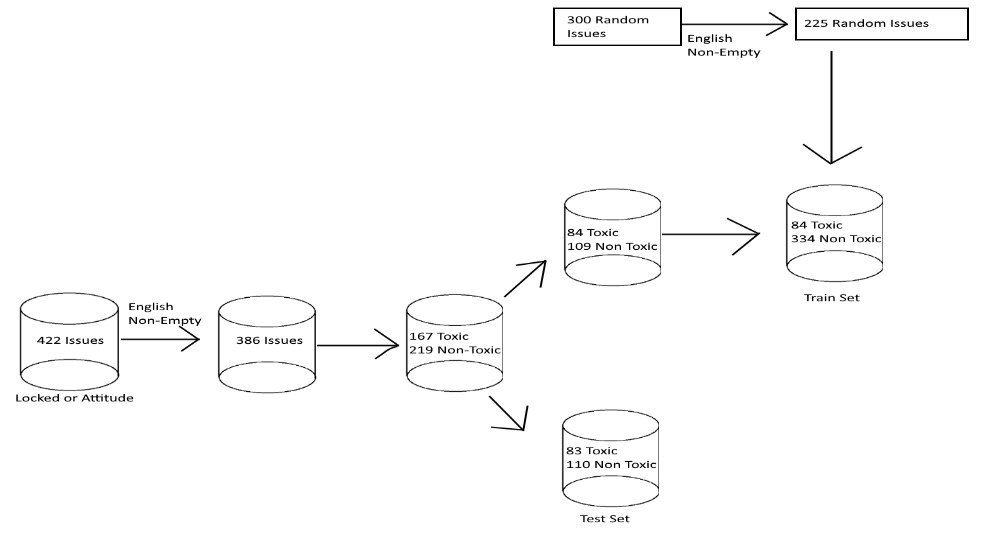
\includegraphics[width=10cm]{data_flow.png}
	\caption{Where data comes from}
\end{figure}

\subsection{Classification Overview} 

We used an SVM model along with two filters that leverage NLP information to classify comments. We run the filters over issues that are classified as toxic to remove possible false positives. After classifying all the comments associated with an issue, we classify the issue as toxic if it contains one or more comments classified as toxic. One toxic comment can derail a conversation and cause it to be toxic, which is why we classify issues in this manner.  

\begin{figure}
	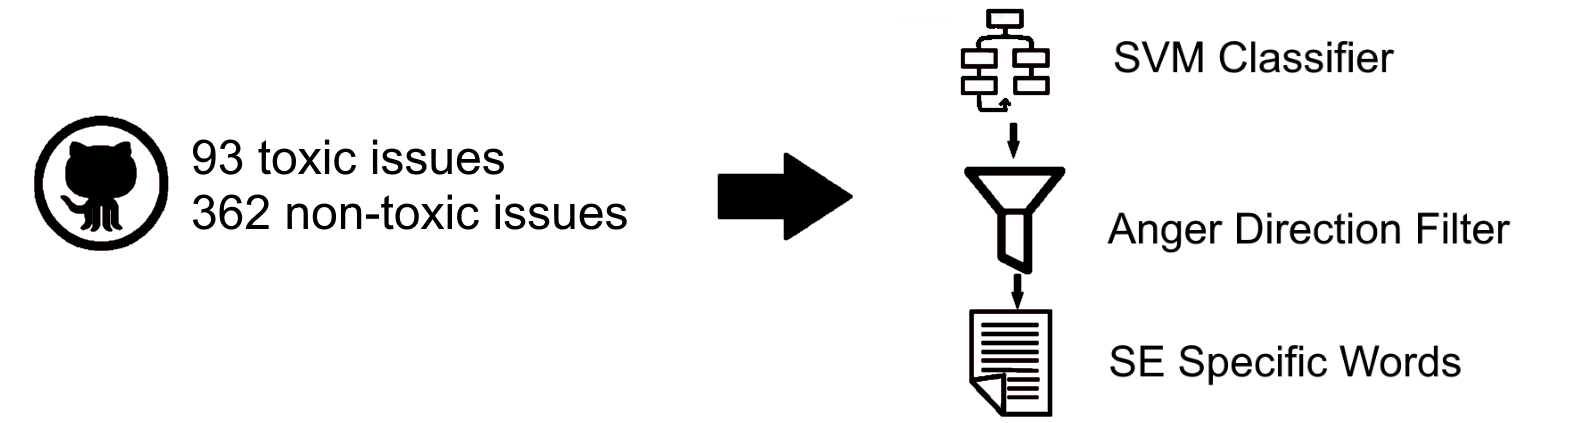
\includegraphics[width=10cm]{pipeline.png}
	\caption{Pipeline}
\end{figure}

\subsection{SVM Classifier}

We removed comments comments that were non-English through the langdetect Python library (CITATION) because we were building a classifier only to classify comments in English. We also removed comments that were empty because there was no text to classify. 

We used an SVM to classify comments as toxic or non-toxic because SVMs are often used for text classification purposes \cite{joachims1998text} and because SVMs outperformed Naive Bayes, Random Forest, and Logistic Regression. 

The SVM uses three types of features: comment metadata, API scores, and text based features. We listed all features in Table I. 

\begin{table}[]
	\begin{tabular}{ p{2cm} p{6cm}} \hline
		\textbf{Feature} & \textbf{Description}                                                                                        \\ \hline
		Num Emojis       & Number of Emojis                                                                                             \\
		Num Urls         & Number of URLs                                                                                              \\ 
		Length           & Length in Characters                                                                                        \\
		Stanford Polite  & Using \cite{danescu2013computational} we give a 0-1 score of politeness, where 0 is the least polite, and 1 is the most polite     \\ 
		Perspective      & Using \cite{perspective}, we give a 0-1 score of how toxic comments are, where 0 is the least toxic and 1 is the most \\
		Subjectivity     & Using TextBlob sentiment, get a 0-1 score of subjectivity, where 1 is the most subjective                   \\ 
		Polarity         & Using TextBlob sentiment, get a -1-1 score of polarity, where 1 and -1 are the most subjective              \\
		NLTK Vader       & Using VADER sentiment analyzer \cite{hutto2014vader}, we find the compound sentiment score                             \\
		TF IDF           & Use TF IDF word frequencies                                                                                 \\ 
		Anger            & Number of words from Anger Lexicon \cite{zhang2018conversations}                                                               \\ 
		Negative         & Number of words from Negative Lexicon \cite{zhang2018conversations} \\  \hline                                                           
	\end{tabular}
\\ 
\caption{List of Features} 
\end{table}


\textbf{Comment Metadata} - We calculated the number of emojis, the number of URLs and the length of the text (in characters), and used these as features for our SVM. We used these features in case there were structural differences between toxic and non-toxic comments.  

\textbf{API Scores} - Existing NLP libraries provide good algorithms for sentiment analysis. Though not designed for Software Engineering, they provide good approximations of sentiment in Software Engineering. We used Google's Perspective API, Stanford Politeness API, NLTK's VADER, and TextBlob's Subjectivity and Polarity. We used these APIs because they give numerical values for the sentiment of a comment. We tried using SentiStrength, but the library is unable to parse large chunks of text (such as entire comments). 

\textbf{Text Based Features} - We store comment text as TF-IDF unigrams, and use these as a feature. We also used several lists of lexicons  \cite{zhang2018conversations}, such as a list of words that indicate anger. We count the number of words from each list, and use each count as a seperate feature. Because of the large number of lexicon lists, we ran all of these together in an SVM classifier, and found that anger leixcons and negative lexicons were the most improtant to predicting toxicity. 

Two challenges were to avoid falsely classifying self-directed toxicity and to deal with words that have a different meaning in Sofware Engineering. To tackle these, we introduced two additional filters. 


\subsection{Anger Direction} 

We filtered out self directed toxicity to avoid falsely classifying phrases such as "I'm so stupid." These phrases typically indicate self loathing rather than toxicity, and would not contribute to the toxicity of a discussion. We used an SVM classifier with unigram features \cite{gachechiladze2017anger}, that classifies the direction of anger as either self, other person or object, and remove all comments where the anger direction is self.  

\subsection{Software Engineering Words} 

Words in software engineering could have different connotations from words in English, such as differences in the meaning of the word abort. To alleviate this issue, we identified words that are significantly more frequent in software engineering using Log Odds with Dirichlet prior \cite{monroe2008fightin}. The method assumes words follow a Dirichlet distribution, and uses that to convert odds to a z-score. We defineds words that were specific to Software Engineering to be words where $\alpha<0.05$ which corresponds to $z>1.645$. Our software engineering corpus came from a random sample of 10K github issues, and our regular English corpus came from the Python library wordfreq \cite{speer2016wordfreq}, which uses seven text sources including the Wikipdia corpus. We replaced each of the Software Engineering specific words with a filler word, so that the sentence structure would not be modified,, re-computed the features for the comment. If the modified comment is classified as non-toxic, then we re-classifed the original comment as non-toxic. 
\section{Validation} 
\subsection{Internal Validation} 
We used 10-fold nested cross validation to tune our hyperparameters and evaluate our model \cite{fearn2010double}. Because of the imbalance in the training dataset, for each train-test split, we adjusted the class weights, with a ratio $r$ between non-toxic and toxic examples, where $r$ is a hyperparameter. We tried using ADASYN and SMOTE, but neither provided any significant improvement over using class weights. We grid searched over hyperparameters $\gamma=\{1,2,2.5,3\}$, $C=\{0.01,0.05,0.1,0.5,1,10\}$ and $r=\{1,1.5,1.75,2,2.25\}$ in our train-validation split. We iteratively added features from Table 1 to find the best feature combination.

To quantify model performance, we used $f_{0.5}$ score, because of the imbalance of our dataset, and because we wanted a precise classifier when run over larger datasets. 

\subsection{Internal Validation Results} 

Our model performed best when using Politeness, Perspective and filtering out Anger Direction and Software Engineering Words, at $\gamma=2$, $C=0.05$, and $r=2$. We obtained a score of $f_{0.5}=0.736$, with a precision of $0.91$ and recall of $0.42$. Figure 2 demonstrates that removing features from our model decreases model performance, while figure 3 demonstrates that adding features to our model does not improve performance.  

\begin{figure} 
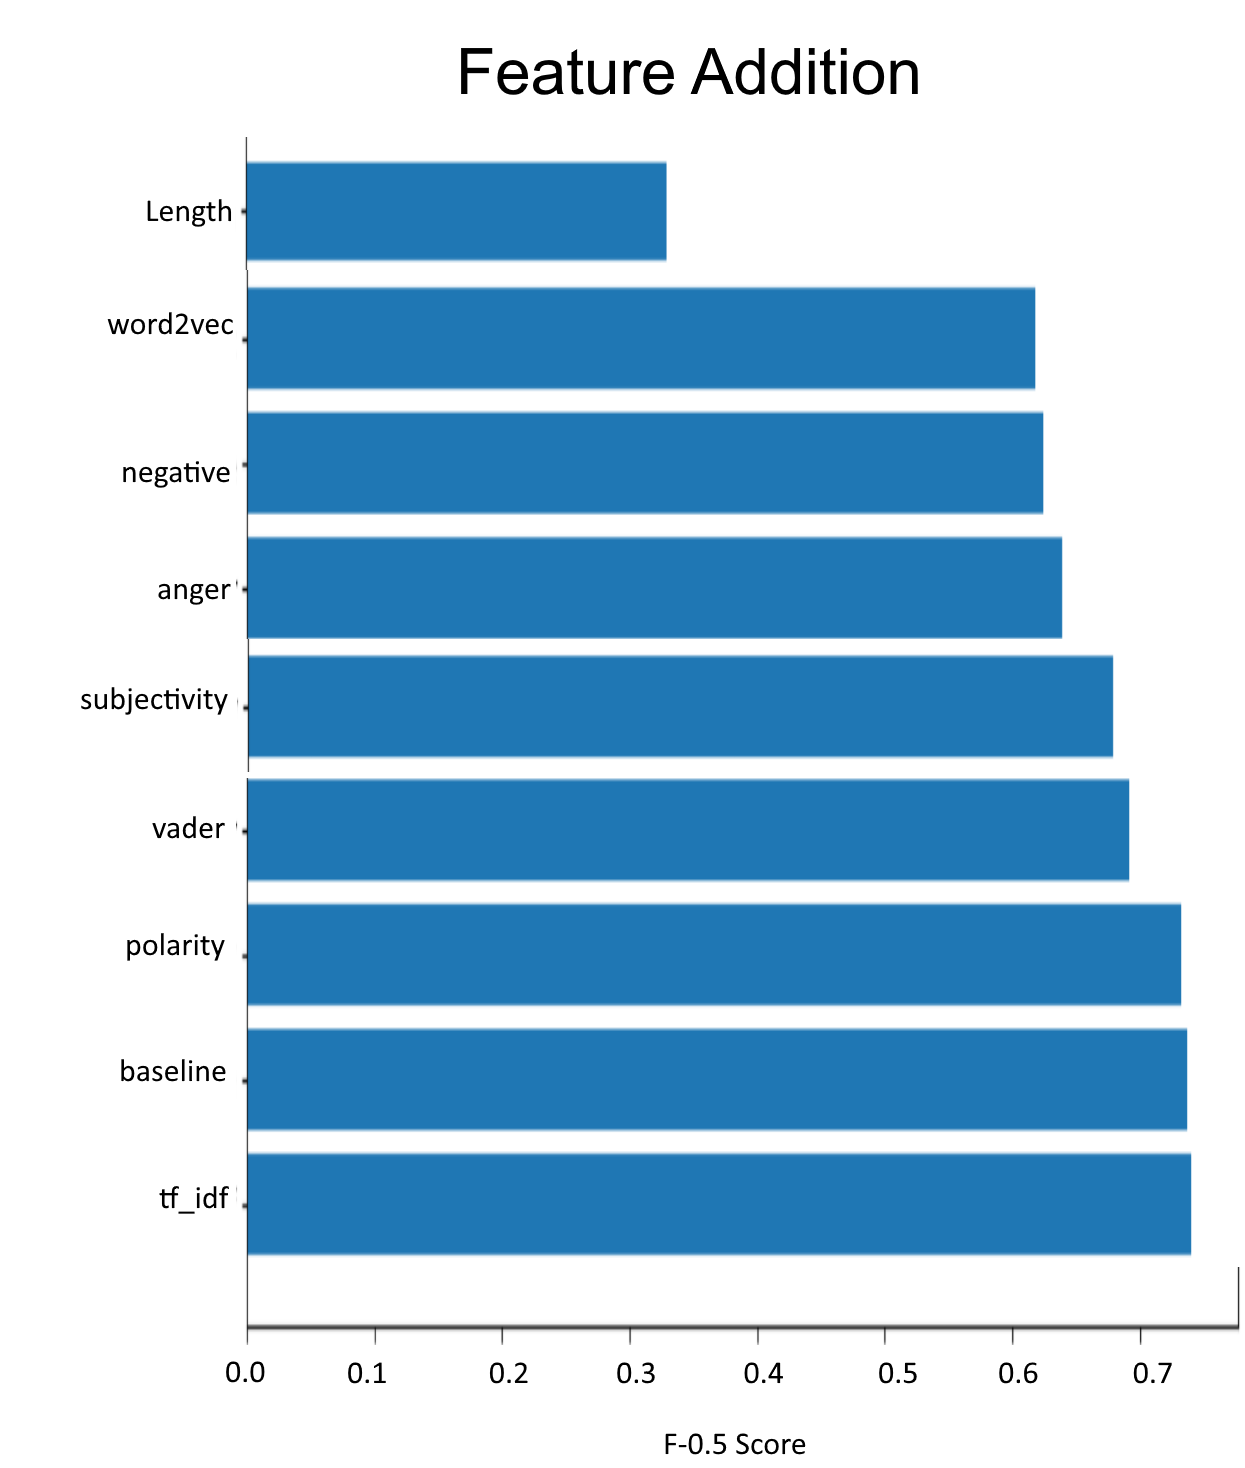
\includegraphics[width=6cm]{feature.png}
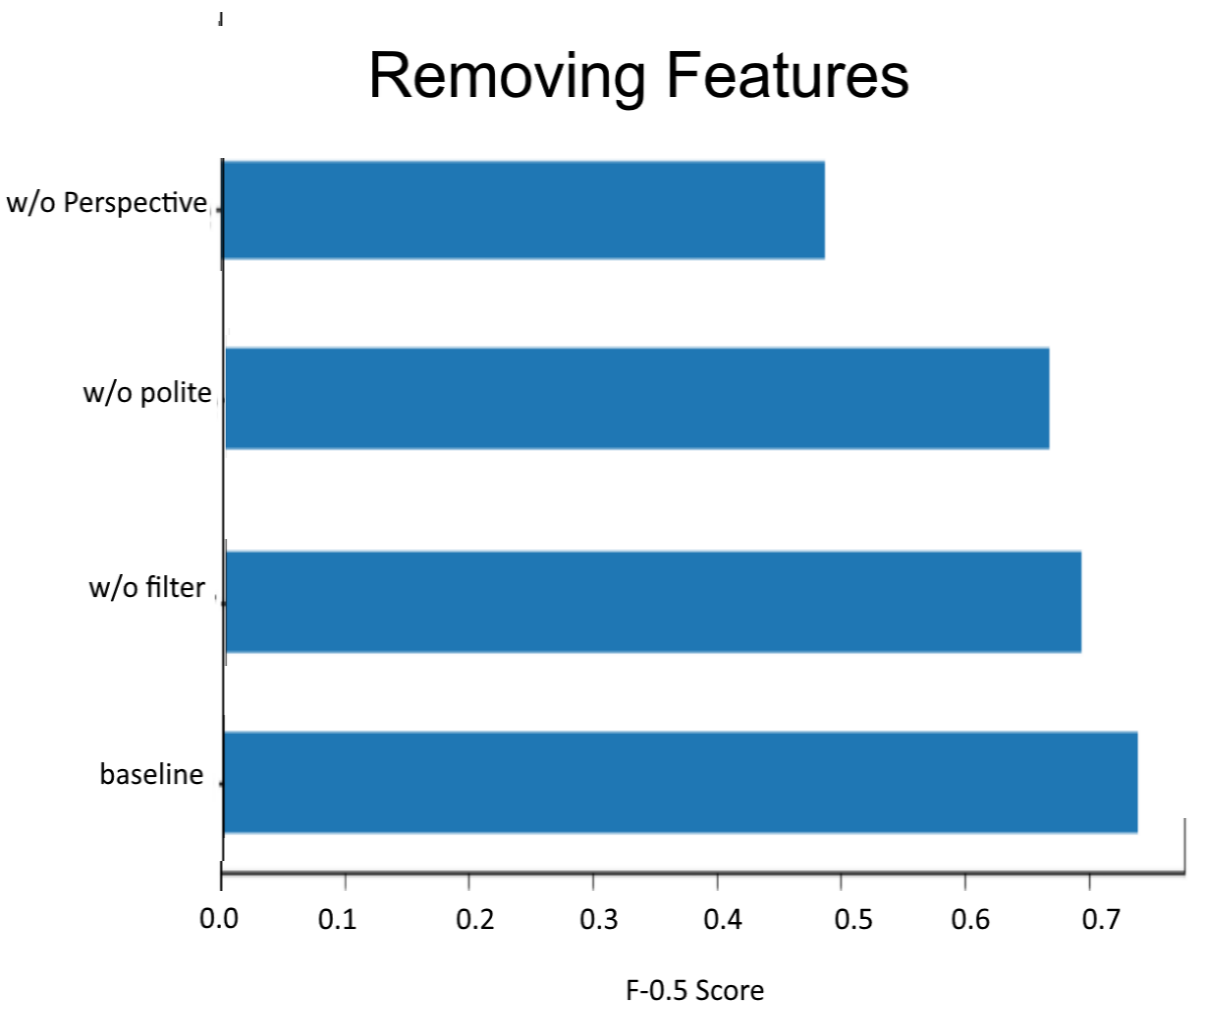
\includegraphics[width=6cm]{remove_features.png}
\caption{Our baseline cannot be improved by adding features, and would be hurt by removing features} 
\end{figure} 

\subsection{External Validation Results} 
We ran our classifier on the held-out labeled examples. We got a recall of 27\% and a precision of 45\%. 

\section{Experiments} 

We used our classifier to identify trends in toxicity. We explored whether the increase in discussion about toxicity corresponded with an actual increase in toxicity. We also explored toxicity across different communities to see whether some communities were more toxic than others. 

\subsection{Toxicity over time} 
There has been more talk recently about burnout in Open Source. We explored whether this increase in dialogue was because of a similar increase in toxicity. 

We explored whether the percentage of toxic comments on Github has increased over time. Because of the infeasibility of classifying every issue on Github, we selected all the issues from each second monday from January 2012-December 2018. We selected the day so to account for potential confounding factors such as the day of the week, or the time of the month. 

We see that toxicity has in fact decreased over the past several years, with an average of 6 toxic comments for every 1000. This implies that, while there has been more discourse on burnout, it might be because of hightened awareness rather than any increase in toxicity. 
 
\begin{figure} 
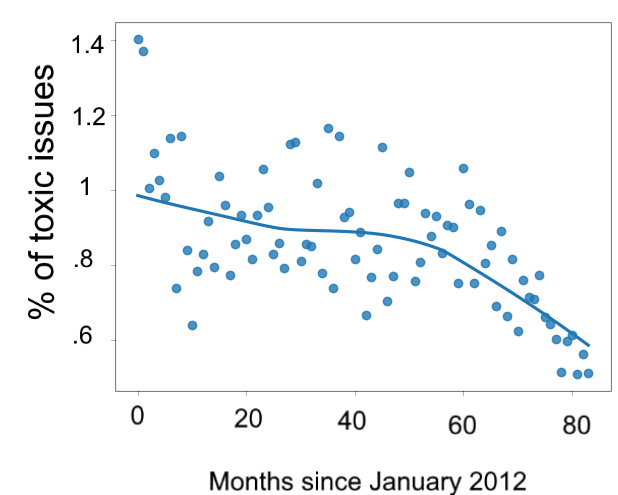
\includegraphics[width=7cm]{toxic_per_month.png}
\caption{Toxicity has decreased since 2012}
\end{figure}

\subsection{Corporate vs. Non-Corporate} 
In recent years, Github has had an influx of projects run or funded by corporate companies. We explored whether this influx has a potentially toxic influence by comparing the toxicity of corporate projects to non-corporate projects. To find corporate issues, we found the top 1000 projects run by some organization or company, removed non-English projects, sorted by number of contributors from that organization, and took the top 100 issues. We wantedp rojects that were not only funded by companies, but also contributed to by members from those companies, because these projects would then have a large corporate influence. None of the top 100 projects were from academic or university sources. We selected all the issues from each of the top 100 projects. 

To find non-corporate projects, we sorted the most popular projects by the number of stars, and selected the top 100 projects that were not run by some company or organization. Again, none of the top 100 were from academic sources. We again selected all the issues from each of the top 100 projects. 

\subsection{Community differences} 
Previous work suggests that there exists cultural differences between communities \cite{bogart2016break}. We used languages as a proxy for communities and explored toxicity differences between issues from projects in seven languages: Python, Java, Javascript, Haskell, Lua, R, and Ruby. We tried to pick a variety of langauges so we could identify what factors affected toxicity. We selected all issues from the 30 most popular projects in each of these languages, and classified each issue as toxic or non-toxic. 

\begin{figure}
	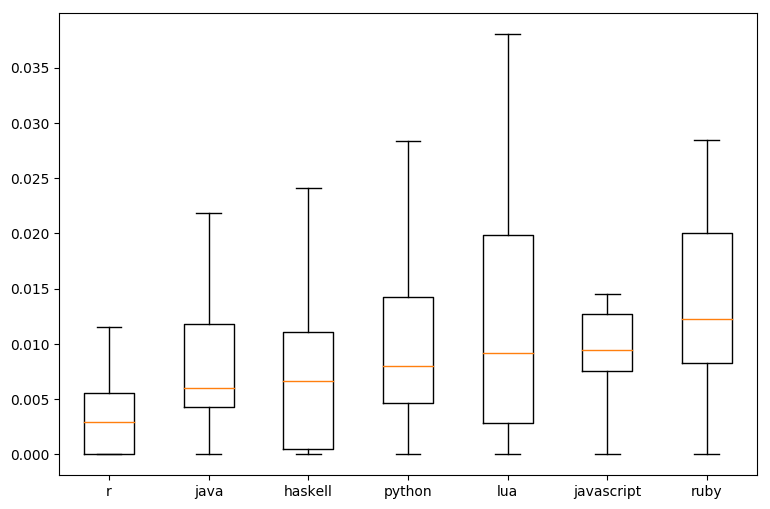
\includegraphics[width=7cm]{box_plot.png}
	\caption{There are differences in toxicity between different languages} 
\end{figure}

We find that R is the project with the least toxicity, and ruby is the project with the most toxicity. This corresponds with the amount of fun that a project has, with the least toxic projects also being those that have the least fun \cite{bogart2016break}. 

\section{Results and Discussion}
Results and Discussion

\section{Threats to Validity}
Threats to Validity


\section{Conclusion}
Conclusion


\bibliographystyle{plain}
\bibliography{bibliography}



\end{document}
